\section{Evaluation and metrics}\label{sec:evalueation}
A pipeline is generally evaluated based on quantitative metrics in machine learning and data science. These metrics are in classification general based on the confusion matrix. An example of a confusion matrix can be seen in \autoref{fig:confusion_matrix}.

\begin{figure}[htb!]
    \centering
    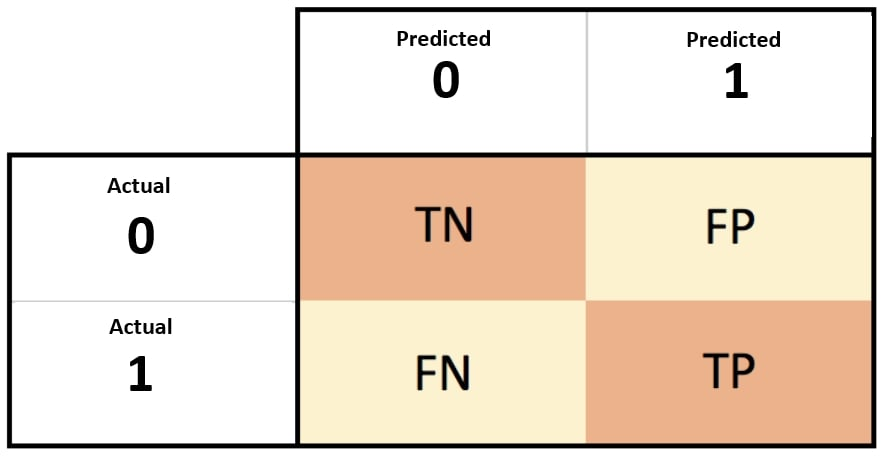
\includegraphics[scale=0.3]{figures/Confusion_Matrix.jpg}
    \caption{Confusion matrix}
    \label{fig:confusion_matrix}
\end{figure}

\autoref{fig:confusion_matrix} has the values: \texttt{TN}, \texttt{FP}, \texttt{FN}, and \texttt{TP}, which stand for True Negative, False Positive, False Negative, and True Positive, respectively.
A confusion matrix represents all an \gls{ml} model's guesses, with the number of guesses placed at the corresponding label where the correctly predicted elements are on the diagonalm, in this case \texttt{TN} and \texttt{TP}~\cite{james-statistical-learning}.

\subsection{Metrics}\label{subsec:metrics}
There are many different metrics, but there are generally four basic ones. These are accuracy, precision, recall, and F1. Outside these, there are more esoteric metrics such as the Mattheus correlation coefficient, Cohen's kappa, and more~\cite{metrics-for-multi}. The following section will describe each of the four basic metrics.

\paragraph{Accuracy} The most straightforward and simple of the metrics is accuracy, as it simply describes the percentage of correct guesses out of all guesses. Accuracy works well in cases where the sizes of the different classes are similar but struggles in cases where one class is much larger than another. In a case where one class is much larger than others, it is possible to achieve very high accuracy by only guessing the larger class, as the larger classes will have a higher weight when compared to the smaller classes~\cite{metrics-for-multi}. The formula for accuracy can be seen in \ref{eq:accuracy}.

\begin{equation}
    Accuracy = \frac{TP + TN}{TP + TN + FP + FN}
\end{equation}\label{eq:accuracy}

\paragraph{Precision} In the case where one class is smaller when compared to the other classes, the precision metric is better suited than accuracy. Precision is an excellent metric to use when the cost of false positives is high, as it measures how many of the positive guesses were positive. Precision can also measure how well the model can be trusted when predicting a class\cite{metrics-for-multi}. The formula for precision can be seen in \ref{eq:precision}.

\begin{equation}
    Precision = \frac{TP}{TP + FP}
\end{equation}\label{eq:precision}

\paragraph{Recall} The third metric is recall, which measures the model's ability to find all the positive samples. In the case of this project, positive samples refer to correctly guessing numbers from the \gls{mnist} dataset.~\cite{metrics-for-multi}. The formula for recall can be seen in \ref{eq:recall}.

\begin{equation}
    Recall = \frac{TP}{TP + FN}
\end{equation}\label{eq:recall}

\paragraph{F1} The last basic metric is F1. F1 is commonly used when both recall and precision are essential; F1 can be considered a weighted average. The formula for F1, is shown in~\cite{metrics-for-multi}. The formula for f1 can be seen in \ref{eq:f1}.

\begin{equation}
    F1-Score = \frac{2}{precision^{-1} + recall^{-1}} = 2\cdot (\frac{precision \cdot recall}{precision + recall})
\end{equation}\label{eq:f1}

These metrics generally get used in a pipeline for hyperparameter tuning and general evaluation of the model's performance. For this project, hyperparameter tuning will generally only use a single metric to focus on to maximize it. In evaluation, the metrics generally explain what the model does well and does not do well~\cite{james-statistical-learning}.






